\documentclass[9pt,twocolumn,twoside]{pnas-new}
% Use the lineno option to display guide line numbers if required.

\templatetype{pnasresearcharticle}

\title{The stability and robustness of the Github network of collaborators}

% Use letters for affiliations, numbers to show equal authorship (if applicable) and to indicate the corresponding author
\author[a]{Jan Kenda}
\author[b]{Andraž De Luisa} 

\affil[a]{University of Ljubljana, Faculty of Computer and Information Science, Ljubljana, Slovenia, jk3977@student.uni-lj.si
}
\affil[b]{University of Ljubljana, Faculty of Computer and Information Science, Ljubljana, Slovenia, ad9366@student.uni-lj.si
}

% Please give the surname of the lead author for the running footer
\leadauthor{Lead author last name} 

% Please add here a significance statement to explain the relevance of your work
%\significancestatement{}

% Please include corresponding author, author contribution and author declaration information
%\authorcontributions{Please provide details of author contributions here.}
%\authordeclaration{Please declare any conflict of interest here.}
\equalauthors{\textsuperscript{1}Both authors contributed equally to this work.}
%\correspondingauthor{\textsuperscript{2}To whom correspondence should be addressed. E-mail: author.two\@email.com}

% Keywords are not mandatory, but authors are strongly encouraged to provide them. If provided, please include two to five keywords, separated by the pipe symbol, e.g:
\keywords{networks $|$ communities $|$ robustness $|$ node centrality} 

\begin{abstract}
    Social networks maintain a fragile equilibrium that can be easily disturbed by removing key individuals called linchpins. 
    This is no less true in the network of Github collaborators \cite{github-graph}. 
    We propose a measure of robustness for social networks, that how vulnerable a network is when it comes to losing a percentage of its key individuals.
    The measure is based on the stability of the community structure of the social network, 
    specifically by finding individuals which we deem most important to maintaining the current social structure.
    We first evaluate the performance of the proposed methods on Lancichinetti–Fortunato–Radicchi benchmark graphs \cite{lfr} and then on the Github network itself.
\end{abstract}

\dates{This manuscript was compiled on \today}
\doi{\url{www.pnas.org/cgi/doi/10.1073/pnas.XXXXXXXXXX}}

\begin{document}

\maketitle
\thispagestyle{firststyle}
\ifthenelse{\boolean{shortarticle}}{\ifthenelse{\boolean{singlecolumn}}{\abscontentformatted}{\abscontent}}{}

% If your first paragraph (i.e. with the \dropcap) contains a list environment (quote, quotation, theorem, definition, enumerate, itemize...), the line after the list may have some extra indentation. If this is the case, add \parshape=0 to the end of the list environment.
\dropcap{S}haring ideas, problems and solutions is a fundamental reason why humans are as advanced as they are today.
This is true in all fields of science: biology, physics, mathematics and potentially even more so in computer science.
With the advancements in technology and specifically the internet in the last couple of decades, 
cooperation between researchers and innovators has never been easier.
This is in large part due to Git and other version control systems, 
which allow both researchers and software developers to interact and collaborate on projects with ease,
in turn leading to faster learning, innovation and development of scientific and technological advancements.

But this network has a big drawback: it is a social network.
And as a social network, it has its linchpins - key members of a society which hold everything together.
Without them the network might fall apart. 
These are the people who introduce others. 
The keys that connect people into a community.
And this is what we are interested in.

If we are able to find a community structure in the GitHub network of collaborators \cite{github-network}, 
we can then try to measure how "well connected" each community is.
Using this measure as a criterion, we can then start looking for linchpins - 
in this case nodes, which if removed, would destabilize the community structure of the network as much as possible.
In the real world social network this means removing individuals that we think contribute most to the development of new ideas and projects.
Not necessarily provide solutions themselves, but by connecting others and creating (or just being the core of) communities, contribute to
further technological advancements the most.

In this paper we analyse the ability of several node centrality measures to highlight these crucial nodes for the robustness of the community structure in social networks.

\section*{Related work}

\paragraph{} A lot of work has been done in detecting communities and evaluating their stability. A quantification of the community structure robustness and the method for its computation is proposed by Karrer et al.\ \cite{karrer-levina}. A somehow similar approach to statistical validation of such partitions of networks into communities has been analysed by Carissimo et al.\ \cite{carissimo}. Both are based on random perturbations of edges in the network, analysing the induced changes in the community structure. Our approach differs from them, as instead on the edges we are more concerned on the importance of single nodes in the communities. 

A node centrality measure for classification of nodes with respect to their importance in the community structure, based on the spectrum of the adjacency matrix, has been recently proposed by Wang et al.\ \cite{wang-yang-fan}.


\section*{Methods and Data}

\paragraph{}For this project we use the data gathered from SNAP \cite{github-graph}, 
which contains a social network of collaborators on Github up until August 2019. 
The nodes of the network are Github users who starred popular machine learning and web development repositories 
(only repositories with at least 10 stars are taken into account).
The edges of the network are their follower relationships. It is an undirected graph.

We start by generating Lancichinetti–Fortunato–Radicchi benchmark graphs with planted communities.
These graphs serve as testing networks for our project.
First we find the communities within the network using various community detection algorithms, such as Louvain \cite{louvain}, Infomap \cite{infomap} and Label propagation \cite{Raghavan-2007}. 

Since the Github network is a social network, the communities are not as well-defined and clearly seperated as is the case with Lancichinetti–Fortunato–Radicchi benchmark graphs.
Because of this, we require algorithms which allow for overlapping communities, 
such as Demon \cite{Demon}, \cite{coscia-rossetti}, which uses a local-first approach to community discovery, or if overlaps are significant,
a $k$-clique algorithm based on \cite{palla-derenyi}, which works by locating all cliques in the network and then identifying communities based on the analysis of the clique-clique overlap matrix.

The next step is measuring how well-connected a community actually is, and how stable is the whole community structure. 
The most basic method would be to simply measure the number of connections between nodes within a community and compare it with the number of connections that lead outside of it.
A more advanced method is to measure the conductance \cite{leskovec-lang-mahoney} of communities of the network.
The stability of the community structure can be estimated from the changes in the number of communities detected, their average size and the number of nodes contained in a community.

Once we have this, we start looking for key nodes that, if removed, would most disturb the community structure of the network.
We do this by employing various methods of node importance.
We use different methods of node centrality, namely degree centrality, closeness, bridgeness, betweenness, pagerank and eigenvector centrality.
We also consider if, instead of removing nodes, we could just remove edges (e.g. sever the collaboration between two users).
For this we calculate the edge betweenness centrality measure for all edges.

Using the above measures as criteria, we start testing by removing the nodes (or edges) with the highest measure and 
again calculating the conductance of communities, their number and average sizes,
or even testing if some communities fall apart into connected components due to the removal of an individual.
As such we aim to find the best measure, or even a combination of measures, to identify key linchpin individuals, 
without which the community structure of a social network would change drastically.

\section*{Results}

%Using the aforementioned measure of finding linchpins, we aim to provide a measure of robustness for social networks,
%with regards to how well they can handle the loss of key individuals. 
%We will test this measure by removing the top $1\%$, $5\%$, $10\%$, $15\%$ and $20\%$ of individuals (based on our selected measure of node importance) 
%and seeing how well the community structure of the graph holds.

Because of the size of the network ($37700$ nodes and $289003$ edges), 
we choose to use degree centrality, eigenvector centrality and pagerank as our measures of node importance.
We use the Demon algorithm to discover overlapping communities, first on the base network and again after each iteration of node removals.
We discard all communities smaller than three nodes.

For each measure of node importance, we start with the base network and then remove $10$ by $10$ most important nodes ($0.026~\%$ of the entire network each step)
and at each step run the Demon algorithm to detect communities.
All three measures yielded similar results. 
It is apparent that there is a small number of very key individual nodes that, when removed, 
cause the entire community structure to change drastically.
The effect can be seen in figures \ref{num_coms}, \ref{avg_size}, \ref{max_size} and \ref{ratio}.

\begin{figure}[!htbp]
    \centering
    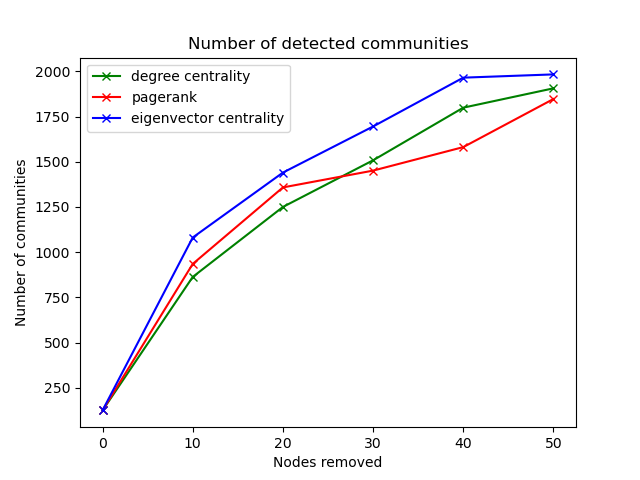
\includegraphics[width=0.9\linewidth]{num_coms.png}
    \caption{The number of detected communites based on how many nodes we remove from the network.
    As can be seen from the graph, as we remove key nodes, communities start to fall apart.
    This is true for all measures of node importance.
    From the fact that the rise in the number of communities with the first removal (from $125$ to $1081$ when using eigenvector centrality)
    is so steep, we can assume there are a few extremely important individuals, who connect several smaller communities into fewer, larger ones.}
    \label{num_coms}
\end{figure}

\begin{figure}[!htbp]
    \centering
    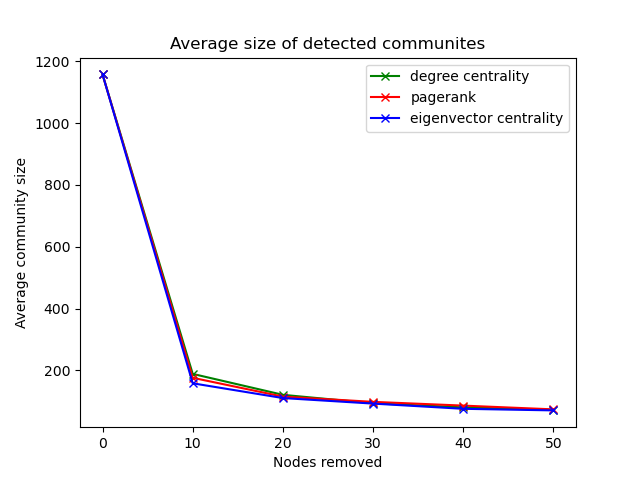
\includegraphics[width=0.9\linewidth]{avg_size.png}
    \caption{The average size of detected communities based on how many nodes we remove from the network.
    All three measures yield extremely similar results, varying only slightly at $10$ removed nodes. 
    The steep drop in the average size is apparent at the $10$ nodes removed mark.}
    \label{avg_size}
\end{figure}

\begin{figure}[!htbp]
    \centering
    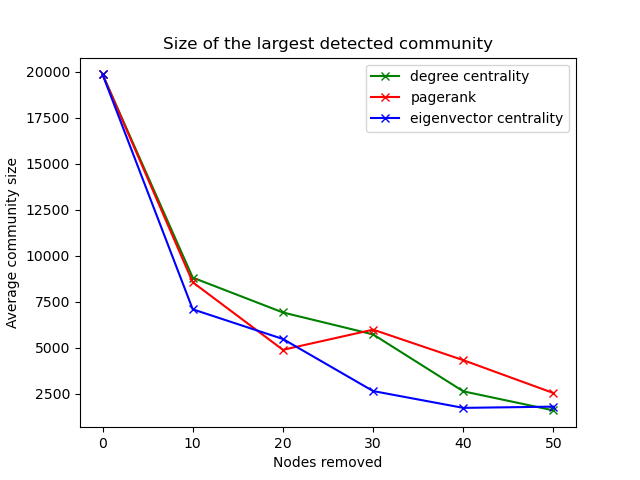
\includegraphics[width=0.9\linewidth]{max_size.png}
    \caption{The size of the largest detected community based on how many nodes we remove from the network.
    From this figure it is apparent that when using different measures of node importance we target different nodes for removal.
    The end results still seem to converge.}
    \label{max_size}
\end{figure}

\begin{figure}[!htbp]
    \centering
    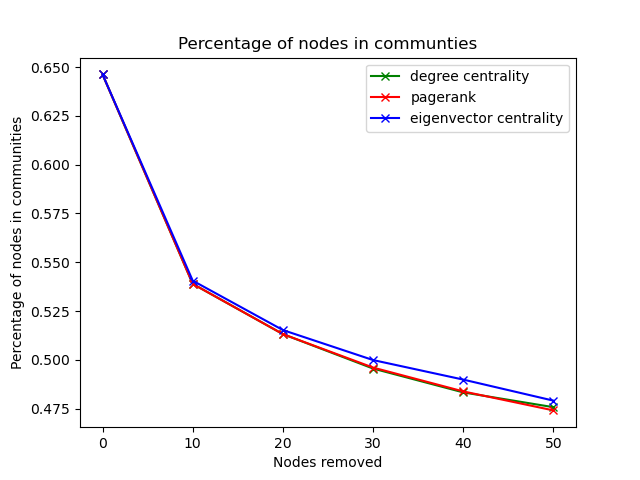
\includegraphics[width=0.9\linewidth]{ratio.png}
    \caption{The percentage of all nodes that are found in communties based on how many nodes we remove from the network.
    All three measures again yielded very similar results.
    In the base network, nearly two thirds of all nodes are in communities.
    After the removal of only $50$ nodes though, less than half of all nodes remain in communities.}
    \label{ratio}
\end{figure}

The number of detected communities seems to be steadily increasing, but it cannot rise forever, so we continue with the nodes removal to check its behaviour.
This time we remove $50$ by $50$ nodes, up to $377$ removed nodes (which is exactly $1~\%$ of the entire network). The results are shown in figure \ref{num_coms_2}.
The other three measures of network robustness 
(average size of communities: figure \ref{avg_size_2}, size of the largest community: figure \ref{max_size_2} and percetage of remaining nodes in communities: figure \ref{ratio_2})
all keep declining at a steady pace.

\begin{figure}[!htbp]
    \centering
    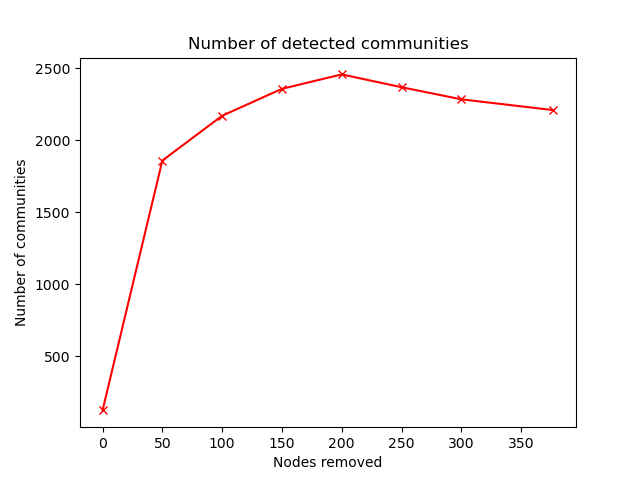
\includegraphics[width=1\linewidth]{num_coms_2.png}
    \caption{The number of detected communites based on how many nodes we remove from the network.
    As we can see, the number of detected communities starts to slowly decline after removing more than $200$ nodes from the network.
    This can be attributed to some communities breaking into parts that are too small to be detected as communities.}
    \label{num_coms_2}
\end{figure}

\begin{figure}[!htbp]
    \centering
    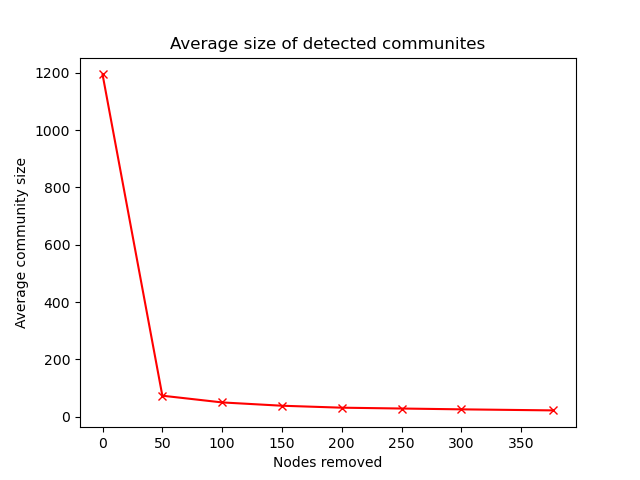
\includegraphics[width=1\linewidth]{avg_size_2.png}
    \caption{The average size of detected communities based on how many nodes we remove from the network.
    It continues to decline at a steady pace.
    While not apparent from the graph, the average size at $377$ removed nodes (avg size of $22.5$) is less than half of that at $100$ removed nodes (avg size of $50.3$).
    }
    \label{avg_size_2}
\end{figure}

\begin{figure}[!htbp]
    \centering
    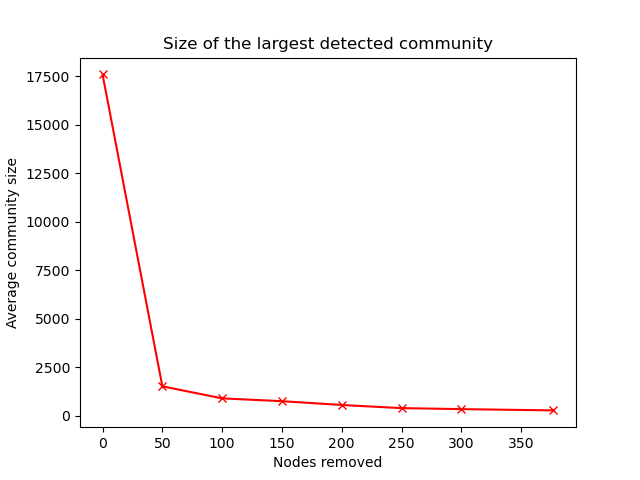
\includegraphics[width=1\linewidth]{max_size_2.png}
    \caption{The size of the largest detected community based on how many nodes we remove from the network. It is steadily decreasing also after the initial drop. At $1~\%$ removed nodes, the largest community contains just $276$ nodes, less than a third than the largest community after the removal of 100 nodes (with 896 nodes).
    }
    \label{max_size_2}
\end{figure}

\begin{figure}[!htbp]
    \centering
    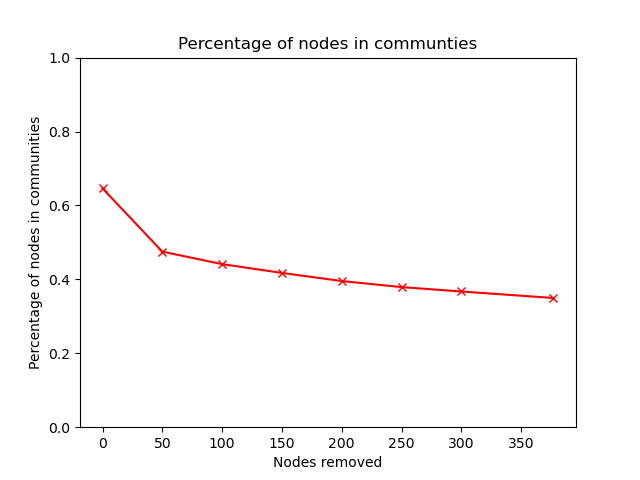
\includegraphics[width=1\linewidth]{ratio_2.png}
    \caption{The percentage of all nodes that are found in communties based on how many nodes we remove from the network.
    At $1~\%$ removed nodes, only $34.9~\%$ of all nodes remaining in communities. This is almost half of the original ($64.6~\%$).
    }
    \label{ratio_2}
\end{figure}

\pagebreak
\section*{Discussion}
Of the three measures of node importance that we used, all three performed similarly. 
We believe that betweenness or bridgeness centralities might perform slightly better, but due to their time complexity, we decided against using them on a network of this size.

The github network is connected. 
What we would like to test further is whether it would be better to seek out and remove articulation points instead of using measures of node importance, thus breaking the network into connected components.
It would also be interesting to test if we can achieve similar community decomposition \emph{without} removing any articulation points,
i.e. keeping the network connected. For this purpose we will need to further explore other node centrality measures.

We also believe that other measures of community quality are needed to evaluate the robustness of the network's partition into communities, hence we will also measure the average conductances, modularities and out-degree fractions.

\begin{table}
    \centering
    \begin{tabular}{|l|l|l|l|l|}
        \hline
        & Eigenv & Degree & Area & Abs diff \\ \hline
        Eigenv & 1 & 0.9811 & -0.6318 & -0.2168 \\ \hline
        Degree & 0.9811 & 1 & -0.7200 & -0.2435 \\ \hline
        Area & -0.6318 & -0.7200 & 1 & 0.5160 \\ \hline
        Abs diff & -0.2168 & -0.2435 & 0.5160 & 1 \\ \hline
    \end{tabular}
    \caption{Correlations between centrality measures}
    \label{tab:cor}
\end{table}


% Bibliography
\bibliography{biblio}

\end{document}